\documentclass[9pt,twocolumn]{extarticle}
\usepackage[a4paper,margin=0.7in,columnsep=0.22in]{geometry}
\usepackage[T1]{fontenc}
\usepackage{lmodern}
\usepackage{microtype}
\usepackage{amsmath}
\usepackage{graphicx}
\usepackage{booktabs}
\usepackage{array}
\usepackage[labelfont=bf,font=footnotesize,labelsep=period]{caption}
\usepackage[numbers,sort&compress]{natbib}
\usepackage{enumitem}
\usepackage{tikz}
\usetikzlibrary{arrows.meta,positioning,fit,shapes.geometric,calc}
\usepackage[hidelinks]{hyperref}
\setlist{nosep,leftmargin=1.3em}
\setlength{\tabcolsep}{3.5pt}
\setlength{\parskip}{0pt}
\setlength{\bibsep}{1pt}
\renewcommand{\bibfont}{\scriptsize}
\newcommand{\bpb}{\textsc{bpb}}

\title{Patch-Aware KV Cache Compression for Byte-Level Language Models:\\A Controlled Study of Attention-Guided, Entropy-Guided and Recency Eviction}
\author{\small Aditya Rayaprolu, Kshitij Gupta, Dhwaj Kishore, Arnab Hazra, Riyazuddin Khan\\[2pt]\small CS F429 Natural Language Processing, BITS Pilani Hyderabad Campus, Group 12}
\date{}

\renewcommand{\normalsize}{\fontsize{9.6}{11.5}\selectfont}
\begin{document}
\normalsize
\maketitle

\begin{abstract}
Language models that consume raw bytes dispense with the tokenizer, that fastidious intermediary, yet they produce sequences some four times longer than BPE does, so that the key-value (KV) cache, the principal bottleneck of deployment, swells in proportion. We build a 13.3M-parameter model of the Byte Latent Transformer (BLT) kind, with patch-granular KV caches, and try cache compression under a disciplined protocol: three seeds per setting, paired bootstrap intervals, random and recency controls, a held-out test split and an analytic reckoning of compute. Four results are of positive worth. (i) Eviction joined to 4-bit quantization retains 7.4\% of a WikiText cache at a cost of $+0.0012$ bits per byte (\bpb). (ii) An online SnapKV-style policy, scored on the model's own attention, outdoes recency in 24 of 24 comparisons. (iii) A cache of fixed size follows documents four times longer than the training context, and 20 PG-19 books, better than resetting the context does, with constant measured memory (0.59 MB against 136.5 MB) and constant time per byte. (iv) The BLT demands 2.8 times fewer FLOPs per byte than a byte-level Transformer of equal width. We also test a seductive proposal: to keep the patches of high next-byte entropy, the very signal the BLT already computes. It is worse than random in 68 and worse than recency in 70 of 72 comparisons, and its penalty swells about tenfold with tenfold training; an error analysis shows that it hoards fragments of one or two bytes. We state what is new, what failed, and what this modest scale cannot reveal.
\end{abstract}

\section{Introduction}
\textbf{The task.} We study language modelling: the prediction of the next symbol of a text from those preceding it, scored in bits per byte (\bpb) on held-out documents. Production systems employ subword tokenizers such as BPE \citep{sennrich2016bpe}. Byte-level models banish the tokenizer, and with it a tribe of failures on rare words, typographical slips, code and foreign scripts \citep{xue2022byt5,yu2023megabyte,slagle2024spacebyte,pagnoni2024blt}; the price is length, a byte sequence being about four times longer than its BPE counterpart (4.0 bytes per token in our data).

\textbf{Why the cache matters.} A decoder, as it generates, hoards the keys and values of every earlier position in every layer. This KV cache, and not the weights, bounds the batch size and the context length at deployment. A byte-level Transformer of our width needs 151 MB per sequence at 16,384 bytes, against 38 MB for BPE (Figure~\ref{fig:memory}). The BLT \citep{pagnoni2024blt} runs its large global Transformer over \emph{patches} of bytes, so that it keeps one cache entry per patch, and it already computes a next-byte entropy to decide where each patch ends.

\begin{figure*}[t]
\centering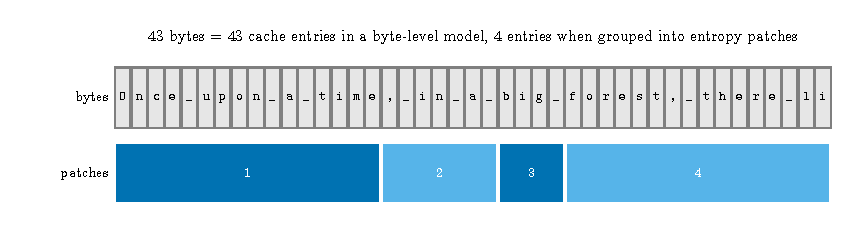
\includegraphics[width=\textwidth]{figures/fig_entries.pdf}
\caption{Why patches relieve the cache. The first 43 bytes of a genuine TinyStories document (spaces shown as underscores) and the four entropy patches into which the model gathers them. A byte-level model stores one key-value entry per byte; the BLT-style model stores one per patch.}\label{fig:entries}
\end{figure*}

\textbf{Why we chose this problem.} Our Part 1 proposal began from three observations: that the KV cache, not the weights, limits how many users may share a GPU and how long a context may run; that tokenizer-free models, alluring for noisy text, code and morphologically rich languages, quadruple that cache; and that the entropy by which the BLT places its patches is computed and then discarded, while existing eviction methods lean on recency or on attention scores computed at runtime. The problem is real, modest enough to study from scratch on a single GPU, and informative whichever way the answer falls.

\textbf{The question.} Might that entropy also adjudicate which patches to keep, or to store at lower precision? It costs nothing extra, so that an affirmative answer would amount to a free compression rule. Related work employs uncertainty to set cache budgets, or as one term of a mixed score, on subword models (Section~\ref{sec:related}); we found no trial of entropy-ranked retention on byte-level models. We tried it against random, recency and attention-based rivals at equal cache bytes. The answer is negative, and the same protocol yielded four positive results (Table~\ref{tab:gain}).

\begin{table*}[t]
\centering\footnotesize
\caption{This work against the previous techniques. ``Previous'' is the Part 2 pipeline (n-gram and BPE Transformer), the standard recency (StreamingLLM-style) cache, context resets for long documents, and a byte-level Transformer. Evidence in the sections named in the last column.}\label{tab:gain}
\begin{tabular}{@{}>{\raggedright\arraybackslash}p{2.5cm}>{\raggedright\arraybackslash}p{4.3cm}>{\raggedright\arraybackslash}p{8.0cm}p{1.6cm}@{}}
\toprule
Aspect & Previous technique & This work & Section\\
\midrule
KV cache at 4,096 bytes & Byte-level Transformer 37.7 MB; BPE Transformer 9.4 MB (hypothetical length); BLT full cache 8.4 MB & 0.2 MB with 64 patches in 4-bit ($+0.0026$ \bpb{} on WikiText); 7.4\% of the BLT cache with 128 patches in 4-bit for $+0.0012$ \bpb & \ref{sec:attn}\\
Eviction rule & Recency with a sink & Online SnapKV-style: better in 24 of 24 comparisons, by 0.0002 to 0.0077 \bpb & \ref{sec:attn}\\
Long documents & Reset the context every 4,096 bytes & Fixed recency cache: $-0.0030$, $-0.0032$, $-0.0008$ \bpb{} (WikiText, 64 patches, three seeds); $-0.0086$ (20 PG-19 books, 256 patches); measured memory constant, time per byte 0.9 ms against a rise to 2.0 ms & \ref{sec:stream}\\
Compute per byte & Byte-level Transformer, 30.9 MFLOPs (1,024 bytes) & BLT 11.1 MFLOPs, 2.8 times fewer (4.75 times at 4,096 bytes); analytic & \ref{sec:flops}\\
Patching & Fixed stride 4 or 5 & Entropy patching is lower in \bpb{} in 3 of 3 same-seed pairs on WikiText validation and test, 67\% of patch starts at word starts; gap about one seed range, so likely rather than established & \ref{sec:base}\\
Modelling quality & Kneser-Ney 4-gram 2.4103; BPE Transformer 1.5200 (WikiText val) & BLT 1.6801 at equal training (behind BPE); 1.29 to 1.31 with ten times more training & \ref{sec:base}\\
Entropy-guided retention (the proposal) & Random and recency & Not an improvement: worse than random in 68 and recency in 70 of 72 comparisons; penalty grows with training & \ref{sec:neg}, \ref{sec:errors}\\
\bottomrule
\end{tabular}
\end{table*}

\textbf{Contributions.}
\begin{enumerate}
\item A BLT-style byte model of 13.3M parameters, compared with a Kneser-Ney byte 4-gram and a 13.8M BPE Transformer, three seeds per setting.
\item A controlled trial of entropy-ranked cache retention on a byte-level patch model (a conjunction we found no earlier trial of), with an unambiguous negative verdict, an anatomy of what the rule actually keeps, and the checks that foreclose the obvious escape routes.
\item Compression that genuinely serves: attention-guided eviction, 4-bit quantization and bounded-memory streaming, with measured memory and time.
\item An online, tested implementation of H2O and SnapKV-style policies over patch caches, an analytic reckoning of compute, quantitative and qualitative error analysis, and a candid account of the difficulties met and the limits that remain.
\end{enumerate}

\section{Literature survey}\label{sec:related}
\textbf{Tokens and bytes.} BPE fuses frequent byte pairs into a fixed vocabulary \citep{sennrich2016bpe}. Token-free models labour on bytes directly: ByT5 \citep{xue2022byt5} shows that a standard Transformer on bytes is competitive in parameters, training compute and inference speed, and more robust to noise; MegaByte \citep{yu2023megabyte} sets a local model within patches and a global model between them; SpaceByte \citep{slagle2024spacebyte} bestows larger blocks after word-boundary bytes such as spaces. The Byte Latent Transformer \citep{pagnoni2024blt} forms patches dynamically from the next-byte entropy of a small byte model, runs a large latent Transformer over them, and reports a FLOP-controlled scaling study to 8B parameters in which patches scale better than tokens at a fixed inference cost. Ours is a simplified BLT: mean pooling in place of cross-attention, no n-gram hash embeddings, and a size of 13.3M.

\textbf{KV cache eviction.} StreamingLLM retains a few initial ``sink'' positions and a recent window, so that a model may stream far beyond its training length \citep{xiao2024streaming}. H2O keeps the ``heavy hitters'', the positions of greatest accumulated attention \citep{zhang2023h2o}. SnapKV selects the positions to which the last queries of the prompt attend \citep{li2024snapkv}. All three act on subword models. We implement recency with a sink, H2O and a SnapKV-style rule (attention from the last 16 patches) as policies over patch entries.

\textbf{KV quantization.} KIVI quantizes keys per channel and values per token to 2 bits without tuning \citep{liu2024kivi}; KVQuant adds non-uniform and outlier-aware schemes for contexts of extravagant length \citep{hooper2024kvquant}. We adopt a humbler symmetric per-vector absmax quantizer and ask only whether the entropy signal can apportion bits.

\textbf{Uncertainty in cache management.} CONF-KV sets the per-step cache budget from the next-token entropy and ranks tokens by attention and recency, with random eviction under the same schedule as a control \citep{li2026confkv}. InfoKV blends predictive entropy and layer-wise representation change with attention scores \citep{kai2026infokv}. Counter-causal surprise scores cached tokens by how well later tokens predict them \citep{gould2026counter}. A learned controller assigns 2 to 16 bits per token from features that include entropy \citep{boroujeni2026bits}. Scratchpad Patching exploits next-byte uncertainty to add temporary slots within byte patches and reports a smaller KV cache \citep{zheng2026scratchpad}. We read the first two in full and only the abstracts of the remaining three, so that our statement of difference from those is provisional. In all of these entropy is one ingredient, or sets a budget; none, to our knowledge, ranks the patches of a byte-level model by entropy alone against random and recency at equal bytes.

\textbf{Relation to the models the public uses.} The general-purpose models in public circulation read BPE subword tokens: Llama 2 employs a 32k vocabulary and a 4k context, Llama 3 a 128k vocabulary and up to 128k tokens of context \citep{touvron2023llama2,llama3team2024}. They already contend with cache growth in the architecture itself: Llama 3 uses grouped-query attention with 8 key-value heads ``to reduce the size of key-value caches during decoding'', which cuts the cache per token fourfold against one KV head per attention head in the 8B model (Figure~\ref{fig:public}). Eviction and quantization of the cache (above) are research methods superimposed on such designs. We study the same bottleneck at a scale one GPU can train from scratch (13.3M parameters, some 600 times smaller than an 8B model) and in the setting these models eschew, raw bytes. Our models do not rival a chat model in capability and we compare no quality; what transfers is the measurement protocol, the policies, and the finding that attention-guided rules serve while the gratuitous entropy signal does not. Since a byte model needs about four times the positions for the same text, its cache predicament is graver, and patching (the BLT) is the architectural remedy on which our compression methods build.

\begin{figure*}[t]
\centering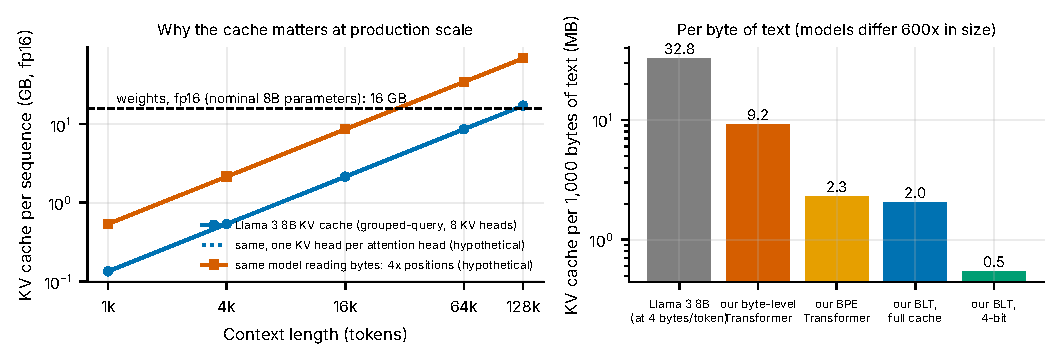
\includegraphics[width=\textwidth]{figures/fig_public.pdf}
\caption{Left: KV cache of a production-scale model grows linearly with context and passes the size of its weights near 128k tokens (computed from the Llama 3 8B configuration: 32 layers, 8 KV heads of dimension 128; fp16). A byte-reading version of the same model would need four times as many positions (hypothetical). Right: our small models per 1,000 bytes of text; the production figure assumes 4 bytes per token and is not comparable in quality, only in cost structure. Configuration and sources in \texttt{configs/analysis/public\_models.json}.}\label{fig:public}
\end{figure*}

\textbf{The classical baseline.} Interpolated Kneser-Ney smoothing \citep{kneser1995improved,chen1999smoothing} is the most accomplished classical n-gram method and furnishes a floor that any neural model ought to clear.

\section{Dataset}\label{sec:data}
\begin{table*}[t]
\centering\footnotesize
\caption{Corpora. Bytes are after normalisation and deduplication. Evaluation sets are fixed and shared by every model. Counts for TinyStories and WikiText-103 are from \texttt{data/processed/*/stats.json} in the Part 2 release.}\label{tab:data}
\begin{tabular}{@{}p{2.3cm}p{4.2cm}p{10.0cm}@{}}
\toprule
Corpus & Domain & Size and use\\
\midrule
TinyStories & Synthetic children's stories & 30,000 train stories (26.7 MB); 21,990 validation; evaluation on the first 500 validation stories (405,231 bytes); no test split\\
WikiText-103 & English Wikipedia articles & 29,002 train articles (526.4 MB, 442 duplicates removed); validation 60 articles (1,129,194 bytes); test 62 articles (1,269,744 bytes)\\
The Stack Smol & Python, Java, JavaScript files & 28,229 files, 15\% of each training batch in the code-mix models; 200 validation files\\
PG-19 & Pre-1919 books & test split, 100 books (40.5 MB); first 100,000 bytes of 20 books, streaming only\\
\bottomrule
\end{tabular}
\end{table*}

\textbf{Sources and fitness.} TinyStories \citep{eldan2023tinystories} is a synthetic corpus of brief stories generated by GPT-3.5 and GPT-4; it trains small models swiftly and offers short documents (about 890 bytes). WikiText-103 \citep{merity2016pointer} holds lengthy Wikipedia articles (about 18 KB apiece), which suit experiments on long-context caches. Both exist in a standard, citable form, and the two sit at opposite poles of difficulty (our baselines reach 0.69 and 1.52 \bpb). The Stack \citep{kocetkov2022stack} (the Smol sample) adds code, since a byte model should not founder on it. PG-19 \citep{rae2019compressive} supplies documents of great length. The first three serve for training and validation; the Wikipedia test split was consulted once, at the end.

\textbf{Limitations and bias.} TinyStories is synthetic, narrow and repetitive, and long training overfits it (37 epochs of a 26.7 MB file, Section~\ref{sec:scale}). WikiText-103 is English and encyclopedic, and so mirrors the topics and registers that Wikipedia covers while neglecting conversational and non-English prose. The Stack sample is permissively licensed code from which only exact duplicates were removed, so that near-duplicate files may render validation code slightly easy. PG-19 is antique literary English, remote from the WikiText-trained models, and its \bpb{} is accordingly high. The release copy of WikiText train is cut to 3,000 articles to keep the demo download at 138 MB (our choice, not a GitHub limit); all reported runs use the full corpus.

\textbf{Preprocessing.} WikiText articles were reassembled from the raw line export, which lacks article boundaries, and placeholder tokens such as \texttt{@-@} were restored. All text is NFC normalised and exact duplicates are expunged. Each split is a single uint8 file of UTF-8 bytes with an offset array; documents are sequestered from one another by a BOS byte and an attention mask; code is split by content hash so that duplicates never straddle splits. Every threshold and hyperparameter was tuned on validation alone.

\section{Method}\label{sec:method}
\begin{figure*}[t]
\centering
\begin{tikzpicture}[font=\scriptsize,>=Stealth,node distance=4mm,
box/.style={draw,rounded corners=2pt,align=center,minimum height=8mm,inner sep=2pt,fill=white},
glob/.style={box,fill=blue!10,draw=blue!60!black},
loc/.style={box,fill=orange!12,draw=orange!70!black},
ent/.style={box,fill=gray!12,draw=gray!70!black},
cache/.style={box,fill=green!15,draw=green!50!black,thick}]
\node[box] (bytes) {bytes\\$x_1\dots x_n$};
\node[ent,right=of bytes] (ent) {entropy model\\3.3M, causal\\$H_i$ per byte};
\node[ent,right=of ent] (patch) {patcher\\boundary where\\$H_i>\theta$};
\node[loc,below=6mm of ent] (enc) {local encoder\\1 layer, width 256\\window 256};
\node[loc,right=of enc] (pool) {mean pool\\per patch,\\linear to 384};
\node[glob,right=of pool] (gl) {global Transformer\\6 layers, width 384\\over patches};
\node[cache,right=of gl] (kv) {KV cache\\one entry per patch\\9,216 bytes (fp16)};
\node[loc,right=of kv] (dec) {local decoder\\2 layers, width 256\\256-way head};
\node[box,right=of dec] (out) {next byte\\$x_{i+1}$};
\node[box,fill=yellow!15,draw=yellow!50!black,below=6mm of kv,minimum width=40mm] (pol) {cache policy: recency, random, entropy,\\H2O, SnapKV-style; 4-bit quantization};
\draw[->] (bytes) -- (ent);
\draw[->] (ent) -- (patch);
\draw[->] (bytes.south) |- (enc.west);
\draw[->] (enc) -- (pool);
\draw[->] (patch.south) -- ++(0,-3mm) -| ($(pool.north)+(0,0)$);
\draw[->] (pool) -- (gl);
\draw[<->] (gl) -- (kv);
\draw[->] (kv) -- (dec);
\draw[->] (dec) -- (out);
\draw[->] (enc.south) -- ++(0,-5mm) -| ($(dec.south)+(0,0)$);
\draw[->,thick,green!50!black] (pol) -- (kv);
\end{tikzpicture}
\caption{The BLT-style model and where the cache policy acts. Bytes are patched by the entropy model, encoded locally, pooled per patch and processed by a global Transformer whose keys and values are the cache; the local decoder predicts each byte from its own encoder state and the global output of earlier patches. The cache policy decides which patch entries are kept and at which precision.}\label{fig:arch}
\end{figure*}

\textbf{The model.} The network is of the BLT kind and bears 13,333,632 parameters. A local encoder (1 Transformer layer, width 256, 4 heads, rotary positions, a causal window of 256 bytes) reads the bytes. The encoder states of the bytes within a patch are mean-pooled and projected to width 384. A global Transformer (6 layers, width 384, 6 heads) runs causally over the patches. A local decoder (2 layers, width 256, window 256) predicts each byte from its own encoder state and the global output of the patches that precede it. The global K and V tensors are the cache we compress: one entry per patch, $2\cdot 6\cdot 384\cdot 2 = 9{,}216$ bytes at fp16. Step-by-step decoding equals the full forward pass to $10^{-5}$ (tested).

\textbf{Patching.} Entropy patching follows the BLT: a separate byte model of 3.3M parameters (4 layers, width 256, window 512) supplies the next-byte entropy $H_i$, and a patch begins where $H_i$ exceeds a threshold tuned on validation to give 4.5 bytes per patch (1.09 nats on TinyStories, 2.17 on WikiText). The decision consults only earlier bytes (tested). Fixed-stride patching (4 or 5 bytes) is the control. Under entropy patching 67.8\% (TinyStories) and 66.7\% (WikiText) of patch starts fall on word starts, against 19.9\% and 16.3\% by chance.

\textbf{Cache policies.} A policy keeps at most $B$ patch entries; the first patch (the sink) and the 8 newest are invariably spared, and every policy chooses among the remainder, so that differences spring from the signal and not from the window. The scores of the old patches are as follows.
\begin{itemize}
\item \emph{recency}: newest first (in the manner of StreamingLLM);
\item \emph{random}: three draws, averaged;
\item \emph{keep high entropy} (the proposal): the mean entropy of the patch, $s_j = |P_j|^{-1}\sum_{i\in P_j} H_i$, the largest being kept;
\item \emph{keep low entropy}: the contrary control;
\item \emph{H2O}: attention received so far, summed over queries, heads and layers;
\item \emph{SnapKV-style}: attention received from the last 16 patches alone.
\end{itemize}
Entropy and recency policies are simulated by masks in a single pass and tested equal to step-by-step decoding in which entries are truly removed. H2O and SnapKV-style need the evicted cache, so \texttt{forward\_online} runs the global layers patch by patch, chooses the entry to discard before the new patch is attended to, and accumulates attention as it is produced (tested for causality and for equality with the full cache at a large budget).

\textbf{Quantization.} Each K and V vector is stored with symmetric absmax scaling at $b$ bits plus one fp16 scale per head. Bytes per entry are 9,216 (fp16), 2,448 (4-bit, 27\%) and 1,296 (2-bit, 14\%). Tier policies grant a fraction of the patches a high width (4 bits) and the rest a low one (2 bits), chosen by recency, by lot, or by entropy, against uniform widths. Eviction and quantization combine by quantizing every entry that survives.

\textbf{Implementation and environment.} Models, policies, quantizer and training loop are our own PyTorch code (\texttt{models/}, \texttt{kvc/}), with rotary positions \citep{su2021roformer}, LayerNorm \citep{ba2016layernorm}, GELU \citep{hendrycks2016gelu}, a 4$\times$ MLP and pre-norm blocks \citep{vaswani2017attention}; training employs AdamW \citep{loshchilov2019adamw} and PyTorch \citep{paszke2019pytorch}. No pretrained checkpoint is used; every weight is trained from nothing. Hyperparameters (BLT): AdamW, learning rate $10^{-3}$, weight decay 0.01, 200 warm-up steps then cosine decay to 10\%, gradient clip 1.0, bf16 autocast, batch 8 of 4,096 bytes, 3,000 steps (30,000 for the long runs), seeds 0 to 2. Entropy model: learning rate $2\cdot10^{-3}$, batch 32 of 1,024 bytes, 3,000 steps, clip 1.0. Seed 0 of the prose-only models was trained on a laptop NVIDIA RTX 4060 (8 GB, Python 3.13, PyTorch 2.9) and the remaining runs on a cluster NVIDIA RTX PRO 6000 (95 GB); the demonstrations and the analyses of Section~\ref{sec:errors} run on CPU.

\textbf{Streaming.} For long documents the fixed-size cache runs 16,384-byte chunks (and, for PG-19, 100,000 bytes one byte at a time with \texttt{BLT.step}) against a baseline that resets the context every 4,096 bytes, the training length.

\section{Experiments}\label{sec:exp}
\subsection{Setup, metrics and baselines}
\textbf{Training budgets.} The principal models see about 98M bytes (3,000 steps); some WikiText code-mix models train for 30,000 steps (about 983M bytes, 1.9 epochs) and at a context of 16,384 bytes. The same checkpoint scores identically on the laptop and the cluster GPU.

\textbf{The metric.} Bits per byte is the total negative log2-probability of a document divided by its byte count. It is indifferent to the tokenizer, so that the 4-gram, the BPE Transformer and the byte models are compared on identical text, and it equals the size per byte that an arithmetic coder driven by the model would attain \citep{deletang2023compression}. Its limits are these: it measures prediction, not downstream use such as retrieval; differences between cache policies are slight (at most 0.03 \bpb), so that every comparison is paired by document and reported with a 95\% bootstrap interval over documents (2,000 resamples); and the Part 2 BPE figure is 0.4 to 0.5\% flattering, because the first token of each 256-token chunk is context only while its bytes are counted (corrected values 0.6978 and 1.5257). Cache size is the mean resident global KV size computed from entry counts and bit widths, and measured on a GPU for recency alone (Figure~\ref{fig:memory}).

\textbf{Baselines.} The classical baseline is an interpolated Kneser-Ney byte 4-gram; the modern one a 13.8M BPE Transformer (6 layers, 6 heads, width 384, 8k vocabulary, 256-token context, 3,000 steps). Cache baselines: the full cache, recency with a sink, random, H2O, SnapKV-style, and uniform 8, 4, 3 and 2 bits. The Transformer was trained before gradient clipping was introduced (clipping gives 0.6826 on TinyStories), so the modern baseline is a trifle handicapped.

\begin{table}[t]
\centering\footnotesize
\caption{\bpb{} on identical documents, lower is better. TS is TinyStories, WT is WikiText-103. First rows are the Part 2 baselines. BLT rows are seed 0, 3,000 steps, validation; the last row is the mean of the three 30,000-step code-mix seeds (1.2949, 1.2983, 1.3118), which saw ten times more training than the baselines.}\label{tab:base}
\begin{tabular}{@{}lrrr@{}}
\toprule
Model & TS val & WT val & WT test\\
\midrule
KN byte 4-gram & 1.8085 & 2.4103 & 2.4381\\
BPE Transformer 13.8M & 0.6939 & 1.5200 & 1.5309\\
Entropy model 3.3M & 0.8438 & 1.6983 & n/a\\
BLT, stride 4 & 0.7726 & 1.7600 & 1.7894\\
BLT, entropy patching & 0.7980 & 1.6801 & 1.6986\\
BLT, entropy, 30k steps & n/a & 1.2983 & n/a\\
\bottomrule
\end{tabular}
\end{table}

\subsection{Baselines and base models}\label{sec:base}
Table~\ref{tab:base} gives the comparison. Every neural model is far ahead of the 4-gram (a gap of 1.0 to 1.1 \bpb{} on TinyStories and 0.65 to 0.9 on WikiText). At equal training the BPE Transformer outscores our BLT-style model on both sets (0.69 against 0.80 on TinyStories, 1.52 against 1.68 on WikiText); ours is smaller, more briefly trained, and lacks the hashed n-gram embeddings and cross-attention of the original BLT, so we claim no victory over BPE at equal training. With tenfold training (a comparison that favours the BLT, the Transformer having kept 3,000 steps) the WikiText code-mix BLT reaches 1.29 to 1.31, and its cache is the one we may compress (below).

Entropy patching against fixed stride, three seeds each (mean full-cache \bpb): on WikiText 1.6958 (entropy) against 1.7347 (stride 4) and 1.7629 (stride 5), entropy patching being lower in all three same-seed pairs and with fewer cache entries per byte than stride 4; on TinyStories 0.8183 against 0.8237 and 0.8521. Seed ranges are 0.056 and 0.028 for entropy patching and 0.135 and 0.044 for stride 4, so the WikiText gap of 0.039 is about the size of a seed range. We call it likely, not established. On TinyStories entropy patching merely ties stride 4. A first single-seed comparison that placed entropy patching 3.3\% behind stride 4 on TinyStories did not survive the seeds and was retired.

\subsection{Entropy-guided eviction: a negative result}\label{sec:neg}
\begin{table}[t]
\centering\footnotesize
\caption{\bpb{} of the seed-0 entropy-patched model under cache budgets (first patch and 8 newest protected). Full cache: 0.7980 (TinyStories), 1.6801 (WikiText). Share of full cache bytes in brackets.}\label{tab:evict}
\begin{tabular}{@{}lrrrr@{}}
\toprule
Budget & recency & random & low ent. & high ent.\\
\midrule
TinyStories 32 (32\%) & 0.8078 & 0.8115 & 0.8089 & 0.8231\\
TinyStories 64 (56\%) & 0.8016 & 0.8033 & 0.8026 & 0.8109\\
WikiText 64 (15\%) & 1.6836 & 1.6860 & 1.6901 & 1.6922\\
WikiText 128 (28\%) & 1.6814 & 1.6833 & 1.6864 & 1.6885\\
\bottomrule
\end{tabular}
\end{table}

\begin{figure}[t]
\centering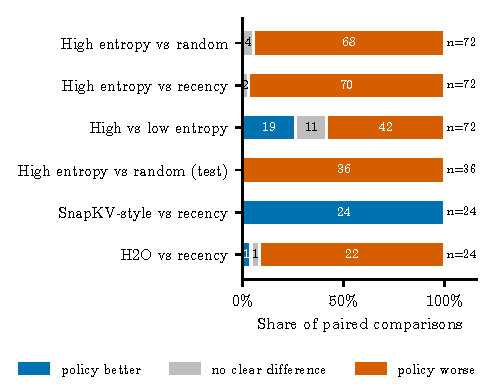
\includegraphics[width=\columnwidth]{figures/fig_scoreboard.pdf}
\caption{Scoreboard of paired comparisons, counted from the result tables. Keeping high-entropy patches is never better than random or recency; the SnapKV-style rule beats recency in every comparison; H2O mostly loses to recency.}\label{fig:score}
\end{figure}
Table~\ref{tab:evict} and Figure~\ref{fig:score} show the proposal losing to random and to recency at every budget. The pattern persists through all the evidence we gathered:
\begin{itemize}
\item Over 72 comparisons (9 models in each of 4 settings, 2 budgets) keeping high entropy is worse than recency with the interval above zero in 70 and indistinguishable in 2, worse than random in 68 and indistinguishable in 4, and never better than either. The paired difference against random is $+0.0003$ to $+0.0245$ \bpb.
\item It holds in every seed, for fixed-stride models (so it is not occasioned by the unevenness of entropy patches), with the code mix, on the WikiText test split (all 36 model and budget cells worse than random and recency), at 16,384 bytes (+0.016 to +0.021 against random at 64 to 512 patches), and for a recency-protected variant (newest half spared, the other half chosen by entropy: worse than recency in 23 of 24 cells).
\item Ablations offer no deliverance (three seeds): the model's own entropy, the first-byte score, the mean score and sink sizes 0 and 4 are worse than random in all seeds on both datasets; the maximum rule is worse in 3 of 3 (WikiText) and 2 of 3 (TinyStories) seeds; only the sum rule on TinyStories is ever better (one seed, $-0.0024$).
\item Keeping \emph{low} entropy beats keeping high entropy in 42 of 72 comparisons, is worse in 19 and ties in 11, so that low-entropy retention is no dependable alternative either.
\item A byte-level cache (one entry per byte) loses far more than a patch cache at equal entry counts: at 32 entries recency costs $+0.2286$ \bpb{} against $+0.0133$ with patches. Patches win per byte of cache; bytes win only with about 4.5 times the cache.
\end{itemize}

\subsection{More training makes the penalty larger}\label{sec:scale}
\begin{figure*}[t]
\centering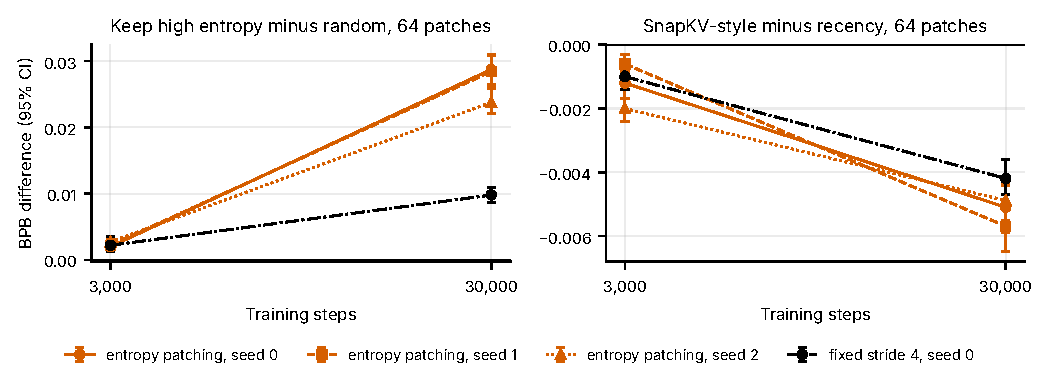
\includegraphics[width=\textwidth]{figures/fig_scale.pdf}
\caption{Ten times more training (3,000 to 30,000 steps, WikiText with code mix) makes the entropy penalty about ten times larger (left) and the SnapKV-style gain several times larger (right). Bars are 95\% bootstrap intervals; three seeds of entropy patching, one of fixed stride.}\label{fig:scale}
\end{figure*}
A natural objection holds that a small, briefly trained model consults its cache but little. WikiText code-mix models trained for 30,000 steps score 1.2949, 1.2983 and 1.3118 \bpb{}, and keeping high entropy costs $+0.0287$, $+0.0284$ and $+0.0238$ against random at 64 patches (against $+0.0020$ at 3,000 steps), every interval excluding zero (Figure~\ref{fig:scale}). Any eviction also costs more (recency at 64 patches costs 0.018 \bpb{} over the full cache, from 0.002), and the fixed-stride model shows the same sign. The TinyStories version overfits (training loss 0.14 nats, validation \bpb{} 1.6493) and is not used. Nor does a longer context redeem the rule: our first 16,384-byte models were under-trained and suggested that the penalty fades, a conclusion retracted after tuning (Section~\ref{sec:challenges}).

\subsection{What works: attention, quantization, bounded memory}
\textbf{Attention-based scoring.}\label{sec:attn} Online, the SnapKV-style rule outdoes recency in all 24 comparisons on the 12 entropy-patched models (by 0.0002 to 0.0077 \bpb, for example $-0.0013$ [$-0.0018$, $-0.0009$] on WikiText code mix, seed 0, 64 patches), and is never worse than its offline approximation. With offline scoring it also beats recency in 33 of 36 test-split cells (the other three tie) and, for the 30,000-step models, by 0.0051, 0.0057 and 0.0049 at 64 patches. Online H2O is worse than recency in 22 of 24: accumulated attention favours old patches that were popular early. The effect is slight (for seed 0 on TinyStories at 32 patches recency costs 0.0098 over the full cache and SnapKV-style recovers 0.0041), but it is the one signal that bested recency, and it is attention, not surprise.

\begin{figure*}[t]
\centering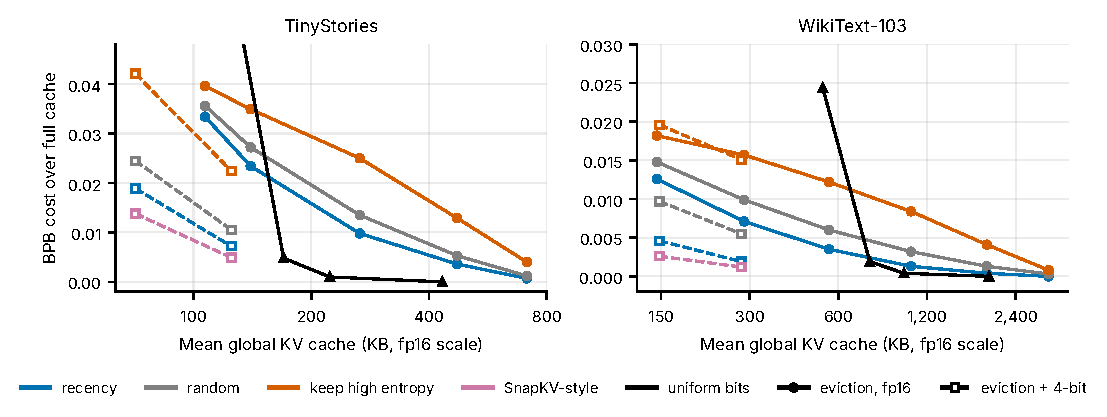
\includegraphics[width=\textwidth]{figures/fig_frontier.pdf}
\caption{Cost over the full cache against cache size (seed-0 eviction and uniform rows from \texttt{comparison.md}; 4-bit rows are the three-seed mean from \texttt{deploy\_combo.md}). Keeping high entropy (orange) is the worst eviction rule at every size and never on the frontier; SnapKV-style with 4-bit (pink, hollow) is the best low-memory point. Uniform 2 bits is off scale.}\label{fig:frontier}
\end{figure*}

\textbf{Quantization and combination.} Uniform 4-bit K and V costs 0.0003 to 0.0014 \bpb{} over fp16 across ten models at 27\% of the bytes (uniform 3-bit 0.0014 to 0.0077, 2-bit 0.022 to 0.111). Entropy-guided precision tiers lose to random and to recency tiers in all ten models. Eviction and 4-bit together, the mean of three seeds, appear in Table~\ref{tab:combo}: a WikiText cache of 128 patches in 4-bit holds 7.4\% of the full cache bytes and costs $+0.0012$ \bpb{} with SnapKV-style eviction ($+0.0019$ with recency), whereas keeping high entropy costs $+0.0151$. No setting that retains high-entropy patches lies on the bytes-against-\bpb{} frontier (Figure~\ref{fig:frontier}).

\begin{table}[t]
\centering\footnotesize
\caption{Eviction with uniform 4-bit K and V, mean of three seeds, cost over the full fp16 cache in \bpb{} (share of full cache bytes). Full cache: 0.8183 (TinyStories), 1.6958 (WikiText).}\label{tab:combo}
\begin{tabular}{@{}lrr@{}}
\toprule
Setting & TinyStories & WikiText\\
\midrule
SnapKV-style, 64, 4-bit & $+0.0049$ (15\%) & $+0.0026$ (3.9\%)\\
recency, 64, 4-bit & $+0.0072$ (15\%) & $+0.0046$ (3.9\%)\\
keep high ent., 64, 4-bit & $+0.0224$ (15\%) & $+0.0196$ (3.9\%)\\
SnapKV-style, 128, 4-bit & n/a & $+0.0012$ (7.4\%)\\
recency, 128, 4-bit & n/a & $+0.0019$ (7.4\%)\\
\bottomrule
\end{tabular}
\end{table}

\begin{figure*}[t]
\centering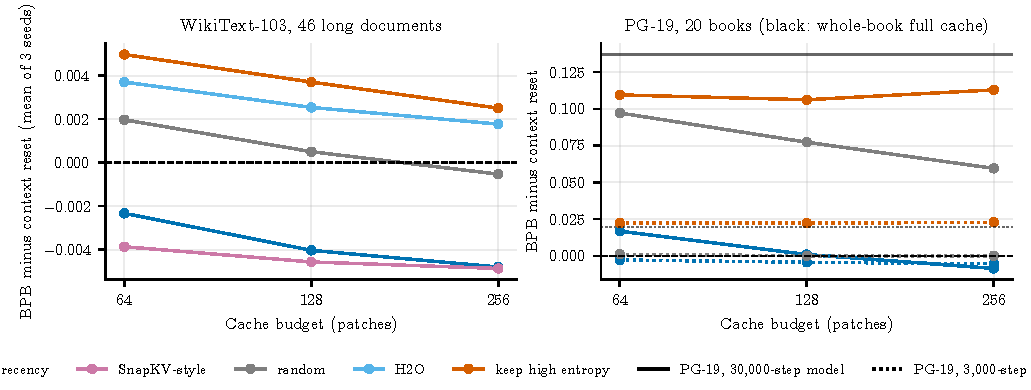
\includegraphics[width=\textwidth]{figures/fig_stream.pdf}
\caption{Bounded-memory streaming. Left: WikiText documents longer than 8,192 bytes decoded in 16,384-byte chunks (patch positions four times beyond training); below zero beats resetting the context every 4,096 bytes. Right: 20 PG-19 books of 100,000 bytes decoded one byte at a time (positions about 22,000). Recency is the only policy that is safe on books; keeping high entropy is worst but is confounded by distance (Section~\ref{sec:stream}).}\label{fig:stream}
\end{figure*}

\textbf{Bounded-memory streaming.}\label{sec:stream} Three WikiText code-mix models trained on 4,096-byte chunks decoded 46 validation documents longer than 8,192 bytes under a fixed patch budget. Recency with 64 patches beats the chunked full-cache baseline in all three seeds (by 0.0030, 0.0032 and 0.0008 \bpb; with 256 patches by 0.0051, 0.0058 and 0.0035), because the reset forfeits the context at every chunk boundary and a small continuous window does not. SnapKV-style is better still at 64 patches (0.0014, 0.0008 and 0.0024 below recency). Random, H2O and keeping high entropy are worse than recency at every budget in all seeds (Figure~\ref{fig:stream}, left). On PG-19, with the 30,000-step model, 256 patches of recency beat the reset baseline by 0.0086 \bpb{} [0.0079, 0.0093] and the whole-book full cache by 0.145; the whole-book full cache is worse than the reset baseline (by 0.137), so the model makes no use of a context 24 times longer than that on which it was trained. Keeping high-entropy patches is $+0.093$ to $+0.122$ worse than recency. To keep old patches is to attend across distances never seen in training, and we did not renumber positions inside the cache as StreamingLLM does, so that PG-19 cannot disentangle a poor entropy signal from poor long-distance attention.

\begin{figure*}[t]
\centering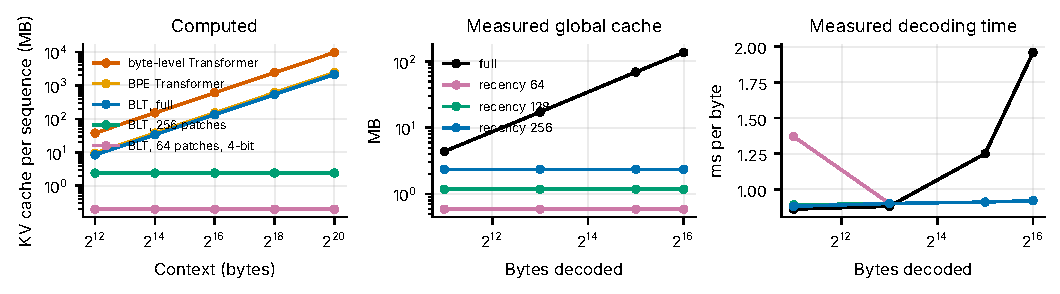
\includegraphics[width=\textwidth]{figures/fig_memory.pdf}
\caption{Cache memory. Left: computed KV size per sequence. Middle and right: measured on a GPU, one stream, real eviction of recency. A bounded cache holds the global cache at 0.59 to 2.36 MB while a full cache reaches 136.5 MB at 65,536 bytes; time per byte stays at 0.9 ms against a rise to 2.0 ms. The first recency point includes warm-up.}\label{fig:memory}
\end{figure*}

\textbf{Memory and speed.} Figure~\ref{fig:memory} gives the measured savings. Certain fixed costs are not reduced: the 786 KB byte-window caches and the entropy model (about 2.1 MB of window cache, 3.3M parameters), so that at 64 patches they exceed the global cache. At full precision the patch cache is about 0.9 times a BPE Transformer cache of the same width, and a byte-level Transformer needs about four times as much.

\textbf{Compute per byte.}\label{sec:flops} The analytic reckoning in the supplement (Table~S1, \texttt{results/part3/flops.md}) is not a measurement. The BLT is cheaper than a byte-level Transformer (11.1 against 30.9 MFLOPs per byte at a context of 1,024 bytes) but \emph{dearer} than the BPE Transformer (7.4), because its local encoder and decoder run on every byte; and it requires the separate entropy model (8.5 MFLOPs per byte) when patches come from entropy, whereupon the total is 19.6. A 64-patch cache pares only the global attention term (0.3 MFLOPs at 1,024 bytes, 1.7 at 4,096). The case for the BLT here is therefore cache memory, not FLOPs.



\textbf{Retrieval.} In a planted-name test (a random name repeated after 400 to 3,000 filler bytes) the models score the same with and without the earlier mention, even at 30,000 steps, so that no policy can be shown to help and nothing about retrieval may be concluded. The entropy rule does retain the name's patches more often than random (45\% against 31\% at 64 patches and 400 bytes), but the model profits nothing from them.

\subsection{Error analysis}\label{sec:errors}
\textbf{The Part 1 pledge.} The proposal promised a split of \bpb{} by entropy, a comparison of code with prose, a retrieval probe, and a scrutiny of generations in which the compressed and full models part company. All four are redeemed: Table~\ref{tab:terc} and Figure~\ref{fig:kept}; \texttt{code\_domain.md} (prose-only models score 7.2 to 7.6 \bpb{} on code, the 15\% code mix 1.75, and entropy retention is still worse than random there, $+0.0036$); the planted-name test (uninformative); and Example 5 below.
We scored 100 TinyStories documents (74,760 bytes, budget 32 patches) and 30 WikiText documents (122,880 bytes, 64 patches) with the seed-0 models, on a CPU. The documents are the first to pass a length filter; the tables describe one seed and are not tests.

\textit{Quantitative.} Table~\ref{tab:terc} apportions the extra loss by the entropy tercile of the patch that holds the byte. Every rule loses most on the high-entropy third, where the full-cache loss is also greatest, but keeping high-entropy patches does not protect those bytes (+0.0392 against +0.0225 for recency on TinyStories; +0.0190 against +0.0062 on WikiText), and it also penalizes the easy bytes (+0.0194 against +0.0080 and +0.0152 against +0.0023 on the lowest third, which holds 57\% and 55\% of the bytes).

The entropy rule retains almost nothing but high-entropy patches (44.6\% and 18.1\% of the highest third survive, none of the lowest), and they are short: the mean kept patch is 1.15 and 1.13 bytes long and 98.0\% and 99.7\% of them have one or two bytes, against 4.46 and 4.47 bytes for recency.

This is a confound of length: a surprising byte often forms a patch of its own, so the mean entropy of a short patch tends to be high. It does not explain the whole result, since the sum rule, which favours long patches, ties random on TinyStories and loses on WikiText (Section~\ref{sec:neg}).

The loss is concentrated: the largest 1\% of bytes carry 30.4\% (TinyStories) and 18.0\% (WikiText) of the extra loss against recency, and entropy is worse than recency on 40.7\% and 51.0\% of bytes and better on 33.1\% and 42.4\%.

\begin{table}[t]
\centering\footnotesize
\caption{Extra loss over the full cache (\bpb) by entropy tercile of the patch holding the byte; share of bytes in brackets.}\label{tab:terc}
\begin{tabular}{@{}llrrr@{}}
\toprule
Set & Tercile & recency & high ent. & low ent.\\
\midrule
TinyStories & lowest (57\%) & $+0.0080$ & $+0.0194$ & $+0.0065$\\
 & middle (32\%) & $+0.0104$ & $+0.0272$ & $+0.0130$\\
 & highest (11\%) & $+0.0225$ & $+0.0392$ & $+0.0253$\\
WikiText & lowest (55\%) & $+0.0023$ & $+0.0152$ & $+0.0035$\\
 & middle (31\%) & $+0.0037$ & $+0.0146$ & $+0.0165$\\
 & highest (14\%) & $+0.0062$ & $+0.0190$ & $+0.0274$\\
\bottomrule
\end{tabular}
\end{table}


\textit{Why? Attention.} We measured the Spearman correlation between the entropy of an old patch (at least 8 patches back) and the attention it receives. It is negative in the middle and upper layers of most models: in all six layers of all three TinyStories seeds ($-0.04$ to $-0.55$), and in layers 2 to 5 of the three prose-only WikiText seeds ($-0.007$ to $-0.39$). In the seed-0 TinyStories model the highest-entropy third of old patches receives about half the attention of the lowest third in layers 1 and 2. The model therefore appears to read predictable patches more than surprising ones, and surprising bytes are handled by the local windows. This is a correlation, not an intervention, and the WikiText code-mix seed 0 model shows the opposite sign in most layers while its eviction result keeps the same sign, so the account is incomplete.



\textit{Qualitative.} In the examples \texttt{|} marks a patch boundary; all are genuine output.

\emph{Example 1, TinyStories document 0 (1,201 bytes, 4.0 bytes per patch).} Boundaries fall before surprising letters and split names: \texttt{R|o|xy. |Ro|x|y |loved to |c|limb.}, while predictable words remain whole patches (\texttt{She |had |never |seen |anything |}). At the last patch the caches (budget 32) hold, for recency, \texttt{played |together |all the |time. |And |Ro|x|y |l|earned that |...} (BPB 0.744, $+0.010$ over full); for keep high entropy, \texttt{\ |s|f|\ |B|s|s|Ro|\ |b|f|b|f|a|s|a|i|...} (0.751, $+0.017$), a sequence of one-letter fragments that keeps \texttt{Ro} but not \texttt{Roxy}; for keep low entropy, \texttt{Once upon a time|, in a |forest, there li|...|never |seen |ried |again, |...} (0.743, $+0.009$), whole words from the opening of the story.

\emph{Example 2, WikiText document 0 (4,096 bytes, budget 64).} The entropy cache at the last patch is \texttt{o|Ho|E|A|O|S|A|a|6|\ |a\ |e|5\ |1|e|e|1|...}: capitals, digits and vowels, and no complete word. BPB is 1.752 ($+0.033$) against 1.725 for recency ($+0.006$), whose cache holds the section on distribution (\texttt{Norway |to |the |A|zores |and |Mo|r|occo}).

\emph{Example 3, where entropy helps.} In TinyStories document 13 the byte \texttt{S} in \texttt{All the animals cheered for [S]am} costs 4.04 bits with the full cache, 7.35 with recency and 3.46 with keep high entropy. The name Sam occurs several times earlier in the story. We did not verify whether the entropy cache held a patch containing the name. Such cases are outweighed on average.

\emph{Example 4, generations that diverge.} Continuing the same prompt greedily with the full cache and with 32 (TinyStories) or 64 (WikiText) patches, recency departs from the full-cache text at byte 17 on TinyStories document 0 (random and keep low entropy at byte 10, keep high entropy at byte 25) and stays with it until byte 65 on WikiText document 1, where random and keep high entropy diverge at the first byte. Greedy text from models this small is repetitive, so this shows where the cache alters the prediction and is not a measure of quality.

\textit{Mitigation.} Keeping high entropy retains short fragments that carry little context and discards the word-sized patches that the decoder uses. Three remedies were tested. Protecting a recency window and allocating half of the slots by entropy reduces the penalty but does not remove it (worse than recency in all 3 seeds at both budgets on TinyStories); ranking old patches by attention (SnapKV-style) outperforms recency in 24 of 24 comparisons; and quantizing every entry to 4 bits instead of evicting costs at most 0.0014 \bpb.



\section{Challenges and how we handled them}\label{sec:challenges}
No separate Part 1 difficulties were recorded; the table covers Parts 2 and 3 (full entries in \texttt{docs/CHALLENGES.md}). Most were discovered by our own consistency checks.

\begin{table*}[t]
\centering\scriptsize
\caption{Difficulties, our responses, and what became of them.}\label{tab:chal}
\begin{tabular}{@{}>{\raggedright\arraybackslash}p{3.3cm}>{\raggedright\arraybackslash}p{6.6cm}>{\raggedright\arraybackslash}p{6.7cm}@{}}
\toprule
Challenge & What we did & Outcome\\
\midrule
Part 2 \bpb{} counted the first token of each chunk, which is context only & Kept the reported numbers for traceability, disclosed the correction (0.6978 and 1.5257), score every byte in Part 3 & BPE number is 0.4 to 0.5\% optimistic; documented, not hidden\\
Seed spread as large as some gaps (0.056 to 0.135 \bpb) & Three seeds for every patching scheme, a stride-5 control, paired bootstrap by document & A single-seed 3.3\% claim retired; the eviction sign holds in every seed\\
Cache byte shares were halved by a counting error & Found when eviction and quantization rows were put in one table (1,669 KB against 839 KB); fixed, all evaluations rerun, tables regenerated & \bpb{} unaffected; shares corrected\\
First 16,384-byte models under-trained (1.89 \bpb) & Tuned learning rate and batch size on validation (1.5843) & Penalty does not fade with context; earlier reading retired. Context length and training amount are not separated\\
TinyStories overfits at 30,000 steps (37 epochs) & Used the WikiText scale-up (1.9 epochs) as the evidence & TinyStories rows reported for completeness only\\
Code data gated; prose models score 7 to 8 \bpb{} on code & Team member login built the set; retrained with a 15\% code mix & Eviction conclusion unchanged; mix costs about 0.05 (WikiText) and 0.09 (TinyStories) \bpb\\
CUDA out-of-memory left a half-written entropy cache while the queue carried on & Caught from the log, cache rebuilt, queue now stops if the cache script fails & No training on corrupt data\\
Offline attention scores only approximate online policies & Built and tested \texttt{forward\_online} & Online SnapKV-style better than recency in 24 of 24\\
Models do not retrieve (planted-name test) & Reported retention rates, drew no retrieval conclusion & Scope stated honestly\\
PG-19 ships as a loading script current libraries do not run & Used a community mirror of the same test split, recorded the substitution & 20 books streamed byte by byte\\
One job at a time, 2-day limit & Checkpoint, handle the pre-limit signal, requeue, resume & Verified end to end under one job id (signal at step 1,864, finish at 24,000)\\
\bottomrule
\end{tabular}
\end{table*}

\section{Scope and limitations}\label{sec:limits}
\begin{itemize}
\item \textbf{Scale.} The models have 13.3M parameters and, for the most part, 3,000 training steps. The 30,000-step models show the same sign with larger effects, but a far larger model might behave otherwise. Ours do not retrieve (planted-name test), so tasks that require retrieval remain untried.
\item \textbf{Data and measurement.} TinyStories has no test split and no usable long-training result; PG-19 rests on 20 books and out-of-domain models. Cache sizes are computed from entry counts, only recency eviction was measured on a GPU, quantization is simulated by rounding, and FLOPs are analytic.
\item \textbf{Seeds.} The 30,000-step fixed-stride model and the 16,384-byte models have one seed apiece; streaming uses three seeds of a single setting; seed 0 of the prose-only models trained on a different GPU (the same checkpoint scores identically on both).
\item \textbf{Mechanism.} The attention and fragment accounts of why entropy fails are correlational; no intervention separates an effect of length, an effect of entropy and a distortion of the global state. On PG-19, to keep old patches is also to attend far beyond the training range, and H2O and SnapKV-style were not run there.
\end{itemize}

\section{Conclusion}
\textbf{New.} A controlled trial of entropy-ranked cache retention on a byte-level patch model, with seeds, paired intervals and a test split; an online, tested implementation of attention policies over patch caches; and measured evidence that a fixed recency or SnapKV-style cache streams documents several times longer than the training context better than a reset does. \textbf{Improved.} Eviction with 4-bit quantization retains 7.4\% of the cache for $+0.0012$ to $+0.0019$ \bpb; SnapKV-style eviction beats recency in 24 of 24 comparisons; memory and time per byte remain constant under a bounded cache; the BLT demands 2.8 times fewer FLOPs per byte than a byte-level Transformer. \textbf{Failed.} The entropy that places patch boundaries is no good arbiter of which patches to keep, and more training makes it worse; the error analysis shows it keeps chiefly fragments of one and two bytes. \textbf{Open.} Whether the results hold for much larger models, or for tasks that require retrieval.

\textbf{Demonstration and reproducibility.} A CPU demonstration (\texttt{scripts/demo.py}) compresses a text, trains a small byte-level model before the viewer's eyes and streams a long text through a genuinely bounded cache (\texttt{docs/demo\_script.md}). Every table and figure regenerates from the commands in the repository README and from \texttt{report/make\_figures.py}.

\bibliographystyle{plainnat}
\bibliography{references}
\end{document}
